% Portfolio RiskQ Poster
\documentclass[final]{beamer}

\usepackage[size=custom,width=121.92,height=91.44,scale=1.0]{beamerposter}
\usetheme{default}

\usepackage{graphicx}
\usepackage{booktabs}
\usepackage{amsmath}
\usepackage{amssymb}
\usepackage{siunitx}
\usepackage{multicol}
\usepackage{enumitem}
\usepackage{tikz}
\usetikzlibrary{calc,positioning}

\setbeamertemplate{caption}[numbered]
\setlist{nosep,leftmargin=1.6em}

% Amber-purple palette (background + logo purple bar style)
\definecolor{AmberPurple}{HTML}{d2c0eb}
\definecolor{LogoPurple}{HTML}{813fcc}
\definecolor{BlockBorder}{HTML}{7061EA}
\definecolor{BlockBG}{HTML}{FFFFFF}
\definecolor{TextDark}{HTML}{000000}
\definecolor{ClassicGreen}{HTML}{1F7A3D}
\definecolor{WarnYellow}{HTML}{F4E04D}
\definecolor{WarnRed}{HTML}{C62828}

\setbeamercolor{normal text}{fg=TextDark,bg=AmberPurple}
\setbeamercolor{background canvas}{bg=white}
\setbeamercolor{block title}{fg=white,bg=LogoPurple}
\setbeamercolor{block body}{fg=TextDark,bg=white}
\setbeamertemplate{blocks}[rounded][shadow=true]
% Add vertical padding to avoid clipped block titles
\setbeamertemplate{block title}{\vspace{0.7ex}\insertblocktitle\strut\par\vspace{0.7ex}}
% Boxed blocks with stronger padding + subtle shadow
\setbeamertemplate{block begin}{
  \par\vskip\medskipamount
  \begin{beamercolorbox}[colsep*=0.9ex,rounded=true,shadow=true,wd=\linewidth,leftskip=0.9em,rightskip=0.9em,sep=0.7ex]{block title}
    \usebeamerfont{block title}\insertblocktitle\strut
  \end{beamercolorbox}
  \begin{beamercolorbox}[colsep*=0.9ex,rounded=true,shadow=true,wd=\linewidth,leftskip=0.9em,rightskip=0.9em,sep=0.9ex]{block body}
}
\setbeamertemplate{block end}{
  \end{beamercolorbox}
  \par\vskip\medskipamount
}
% Make bullets visible and readable
\setbeamerfont{itemize/enumerate body}{size=\normalsize}
\setbeamerfont{itemize/enumerate subbody}{size=\normalsize}
\setlist[itemize]{leftmargin=2.2em,label=\textcolor{LogoPurple}{\large$\blacktriangleright$}}
\setlist[itemize,2]{leftmargin=2.2em,label=\textcolor{LogoPurple}{\normalsize$\bullet$}}

% Ombre background (top white to bottom purple)
\setbeamertemplate{background}{
  \begin{tikzpicture}[remember picture,overlay]
    \path[shade, top color=white, bottom color=AmberPurple]
      (current page.south west) rectangle (current page.north east);
  \end{tikzpicture}
}

\graphicspath{{../poster/}{../experiments/plots/}}

% Title bar similar to the example
\setbeamertemplate{headline}{
  \vspace{0.8cm}
  \begin{center}
  \begin{tikzpicture}
    \node[draw=LogoPurple,fill=LogoPurple,rounded corners=10pt,line width=0pt,inner sep=14pt,minimum width=0.93\paperwidth] {
      \begin{minipage}{0.9\paperwidth}
        \centering
        {\Large\bfseries Portfolio RiskQ}\\[0.15cm]
        {\large Fast Tail Risk Estimation via Discretized IQAE}\\[0.2cm]
        {\large Emily Berlinghoff \quad Amir Orfali}\\[0.1cm]
        {\normalsize Western University \quad Western Quantum Club}
      \end{minipage}
    };
    \node[anchor=west] at ($(current bounding box.west)+(0.6cm,0cm)$)
      {
\includegraphics[height=4.2cm]{wqc.png}};
    \node[anchor=east] at ($(current bounding box.east)+(-0.6cm,0cm)$)
      {
\includegraphics[height=4.2cm]{uwo.png}};
  \end{tikzpicture}
  \end{center}
  \vspace{0.6cm}
}

\begin{document}
\begin{frame}[t]
\begin{columns}[t,totalwidth=\linewidth]

% Left column
\begin{column}{0.31\linewidth}
\begin{block}{Introduction}
Risk teams need reliable VaR/CVaR under tight compute budgets, especially when tail behavior drives capital decisions. We present a classical-to-quantum pipeline that preserves the same loss distribution, tail threshold $\ell$, and histogram while enabling IQAE-based tail probability estimation. The goal is a faster tail estimate with clear, auditable outputs that remain interpretable to non-quantum stakeholders.
\end{block}

\begin{block}{Background}
\begin{itemize}
    \item VaR = loss quantile at confidence $\alpha$; CVaR = expected loss beyond VaR.
    \item Tail threshold $\ell$: cutoff defining the tail region used for CVaR and tail probability.
    \item Portfolio loss: $L = -w^\top r$; tail probability: $p = \mathbb{P}(L \ge \ell)$.
    \item Discretization: map losses into $2^n$ bins to create a quantum-ready histogram.
    \item IQAE: estimates tail probability from the discretized distribution.
    \item Using the same $\ell$ and histogram keeps classical vs quantum comparisons fair.
\end{itemize}
\end{block}

\begin{block}{Objectives}
\begin{itemize}
    \item Build a working classical risk engine and dashboard MVP.
    \item Add discretization and tail-mask generation.
    \item Deliver a small-scale IQAE simulator with resource reporting.
    \item Quantify feasibility limits via resource-aware IQAE experiments.
    \item Communicate results through stakeholder-friendly visuals.
\end{itemize}
\vspace{0.3em}
The emphasis is on a complete, inspectable pipeline that supports both classical validation and quantum-oriented estimation.
\end{block}

\begin{block}{Models \& Materials}
Implementation uses Python with NumPy and Pandas for numerical work, a FastAPI backend for serving risk metrics, and a Streamlit + Plotly front end for interactive visualization.
\begin{itemize}
    \item Gaussian return model; optional crash-mixture scenario.
    \item Nested Monte Carlo for regime uncertainty.
    \item Histogram-based discretization for quantum mapping.
    \item Backend toggle: classical vs quantum comparison path.
\end{itemize}
\end{block}

\begin{block}{Methodology}
\textbf{\large Nested Monte Carlo (loss samples)}

Draw returns from a Gaussian model, then compute portfolio loss as the weighted negative return.
\begin{align*}
    r \sim \mathcal{N}(\mu,\Sigma), \quad L = -w^\top r
\end{align*}

\textbf{\large Tail metrics}

VaR is the loss quantile at level $\alpha$; CVaR averages losses beyond VaR.
\begin{align*}
    \text{VaR}_{\alpha} &= Q_{\alpha}(L) \\
    \text{CVaR}_{\alpha} &= \mathbb{E}[L \mid L \ge \text{VaR}_{\alpha}]
\end{align*}
\vspace{0.4em}

\textbf{\large Discretization}
\begin{itemize}
    \item Bin losses into $2^n$ intervals.
    \item Produce edges, probabilities, tail mask.
    \item Bootstrap error estimate for bin stability.
    \item Bin counts $n_i$ define histogram probabilities $p_i$; tail probability is the sum over tail bins.
\end{itemize}
\begin{align*}
    p_i &= \frac{n_i}{N}, \quad \sum_i p_i = 1, \quad \hat{p} = \sum_{i \in \text{tail}} p_i
\end{align*}
\vspace{0.4em}

\textbf{\large IQAE (simulator)}
\begin{itemize}
    \item Uses Grover iteration schedule to amplify tail states.
    \item Returns estimate with confidence interval.
    \item IQAE probes multiple Grover powers $m$ to infer $p$ from amplified measurements.
\end{itemize}
\begin{align*}
    p &= \sin^2(\theta), \quad p_m = \sin^2((2m+1)\theta)
\end{align*}
\end{block}

\end{column}

% Middle column
\begin{column}{0.35\linewidth}

\begin{block}{System Pipeline (Schematic)}
\begin{center}
\begin{tikzpicture}[
    node distance=1.35cm,
    every node/.style={font=\small},
    classicbox/.style={draw=ClassicGreen,rounded corners=4pt,fill=ClassicGreen!12,inner sep=5pt,minimum height=1.0cm},
    quantumbox/.style={draw=LogoPurple,rounded corners=4pt,fill=LogoPurple!12,inner sep=5pt,minimum height=1.0cm},
    arrow/.style={-stealth,thick,color=LogoPurple},
    iconclassic/.style={draw=ClassicGreen,fill=ClassicGreen!15,circle,inner sep=1.6pt,font=\scriptsize},
    iconquantum/.style={draw=LogoPurple,fill=LogoPurple!15,circle,inner sep=1.6pt,font=\scriptsize}
]
  \node[classicbox] (data) {Market Data};
  \node[classicbox, right=of data] (calib) {Calibration $(\mu,\Sigma)$};
  \node[classicbox, right=of calib] (mc) {Nested MC};
  \node[classicbox, right=of mc] (hist) {Histogram $2^n$};
  \node[quantumbox, right=of hist] (iqae) {IQAE};

  \node[iconclassic, above=0.15cm of data] {D};
  \node[iconclassic, above=0.15cm of calib] {M};
  \node[iconquantum, above=0.15cm of iqae] {Q};
  \node[iconclassic, above=0.15cm of hist] {UI};

  \draw[arrow, color=ClassicGreen] (data) -- (calib);
  \draw[arrow, color=ClassicGreen] (calib) -- (mc);
  \draw[arrow, color=ClassicGreen] (mc) -- (hist);
  \draw[arrow, color=LogoPurple] (hist) -- (iqae);

  \node[classicbox, below=0.9cm of mc] (metrics) {VaR / CVaR};
  \draw[arrow, color=ClassicGreen] (mc) -- (metrics);
  \node[classicbox, below=0.9cm of hist] (tail) {Tail Mask};
  \draw[arrow, color=ClassicGreen] (hist) -- (tail);
\end{tikzpicture}
\end{center}
Market data calibrates $(\mu,\Sigma)$, nested MC yields losses, and discretization builds a $2^n$ histogram and tail mask in the \textcolor{ClassicGreen}{classical} pipeline. IQAE then estimates tail probability in the \textcolor{LogoPurple}{quantum} stage.
\end{block}

\begin{block}{Analysis \& Results}
\begin{itemize}
    \item Validated probability normalization and tail-mask correctness.
    \item Compared IQAE estimates to true tail probability on toy data.
    \item Tracked resource usage (qubits, depth, 2Q gates, oracle calls).
    \item Compared classical vs quantum using the same $\ell$ and histogram.
    \item Discretization tests passed (prob sums to 1, mask correctness).
    \item IQAE toy test estimates matched true tail probability.
    \item Dashboard showed VaR/CVaR and tail-highlighted histogram.
    \item Backend toggle enabled classical vs quantum side-by-side comparison.
    \item Difference fields (abs/rel error) were reported in API/ UI.
\end{itemize}
\end{block}

\begin{block}{Key Contribution}
We present a classical-to-quantum VaR/CVaR workflow that uses a discretized histogram and tail mask to enable IQAE comparison against nested Monte Carlo. We also map feasibility boundaries for NISQ constraints and validate the pipeline in a production-style dashboard.
\end{block}

\begin{block}{Experiment Visuals}
These plots summarize accuracy tradeoffs across classical sampling, quantum query cost, discretization resolution, and noise sensitivity. We report absolute tail-probability error against a known baseline, highlighting where additional compute yields diminishing returns and where noise dominates estimation error.
\vspace{0.3em}
\begin{center}
\begin{minipage}[t]{0.48\linewidth}
    \centering
    \textbf{Classical Error vs Paths}\\[0.2em]
    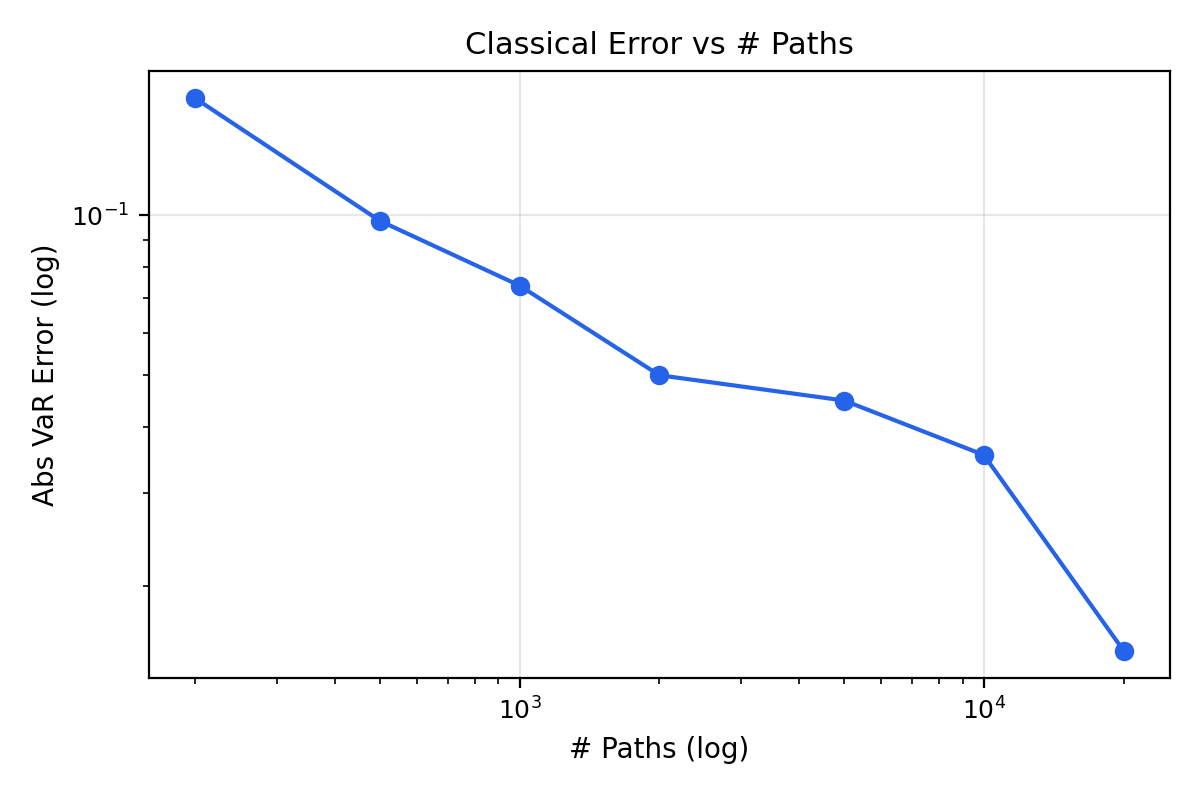
\includegraphics[width=\linewidth]{classical_error_vs_paths.png}
    \\[-0.2em]
    {\scriptsize\colorbox{LogoPurple!15}{\strut Takeaway:} \emph{VaR error falls as $1/\sqrt{N}$; 10k+ paths stabilizes tails.}}
\end{minipage}\hfill
\begin{minipage}[t]{0.48\linewidth}
    \centering
    \textbf{Quantum Error vs Oracle Calls}\\[0.2em]
    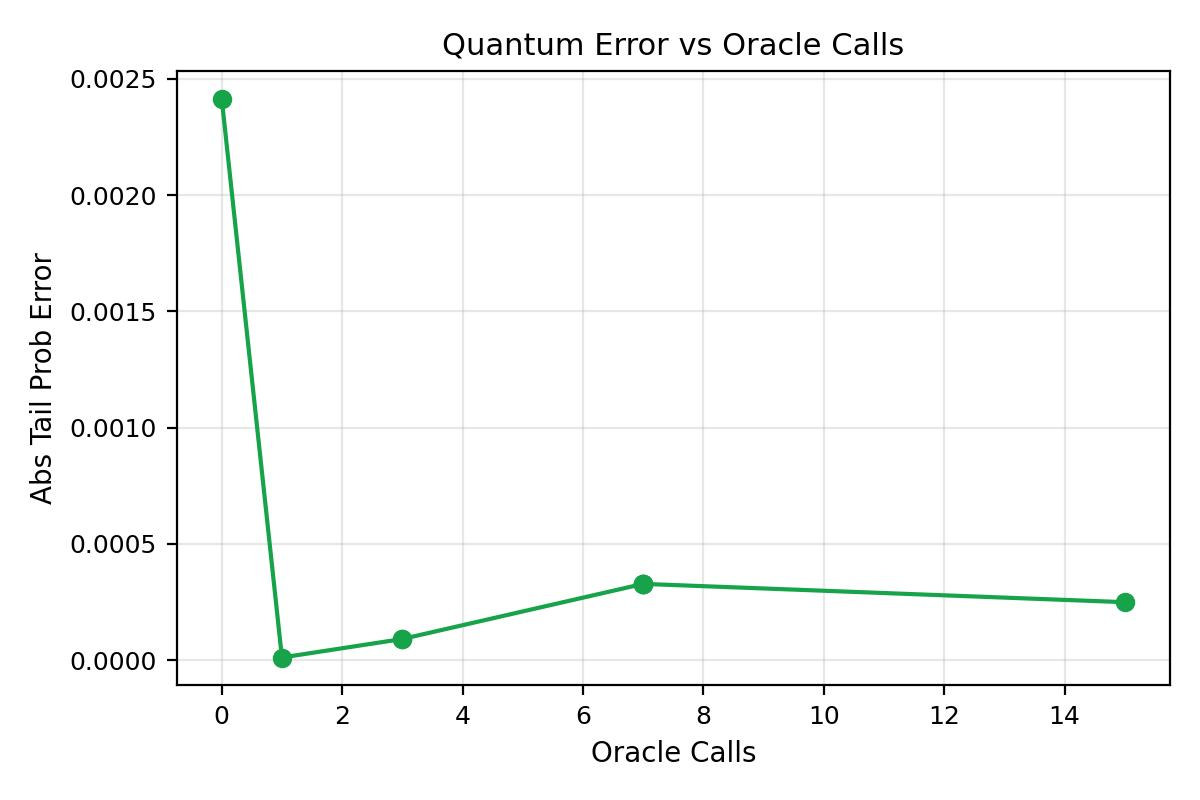
\includegraphics[width=\linewidth]{quantum_error_vs_oracle_calls.png}
    \\[-0.2em]
    {\scriptsize\colorbox{LogoPurple!15}{\strut Takeaway:} \emph{Sub-1\% tail error in a few Grover rounds.}}
\end{minipage}

\vspace{0.3em}

\begin{minipage}[t]{0.48\linewidth}
    \centering
    \textbf{Error vs Discretization Bits}\\[0.2em]
    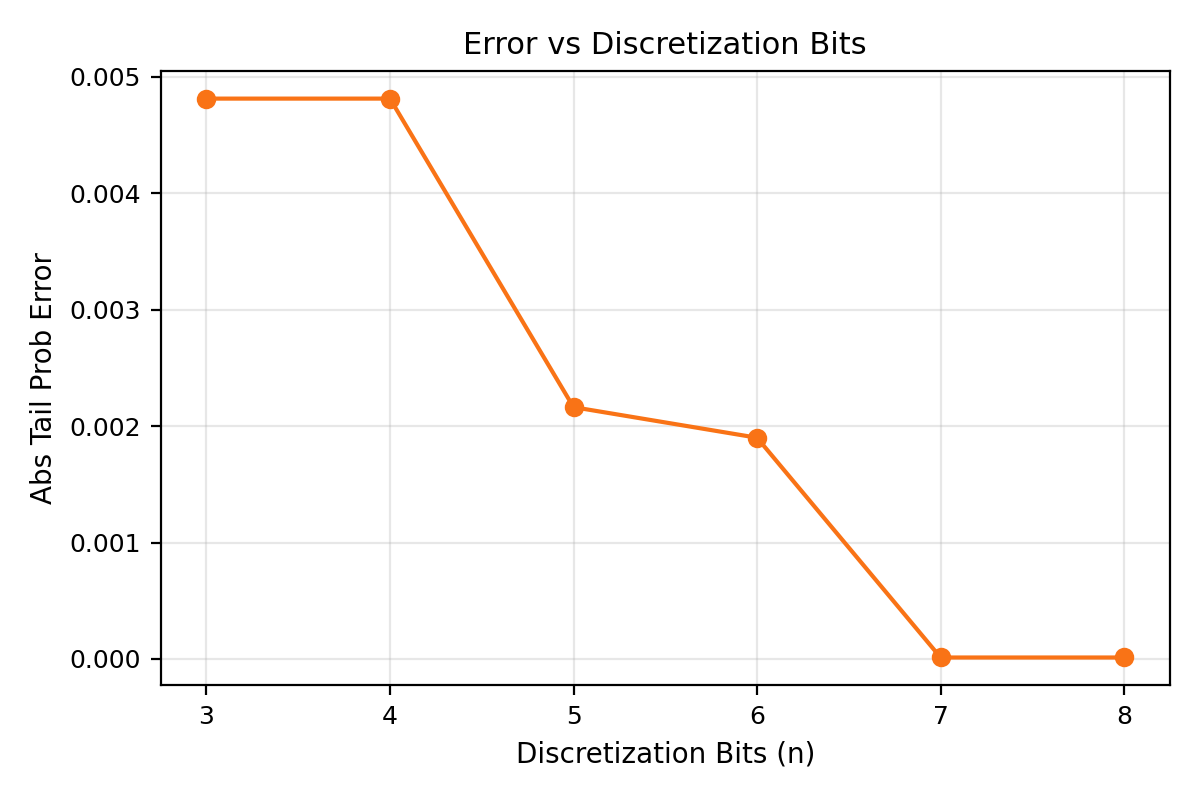
\includegraphics[width=\linewidth]{error_vs_discretization_bits.png}
    \\[-0.2em]
    {\scriptsize\colorbox{LogoPurple!15}{\strut Takeaway:} \emph{Gains taper beyond 6--7 bits (binning bias).}}
\end{minipage}\hfill
\begin{minipage}[t]{0.48\linewidth}
    \centering
    \textbf{Error vs Noise Level}\\[0.2em]
    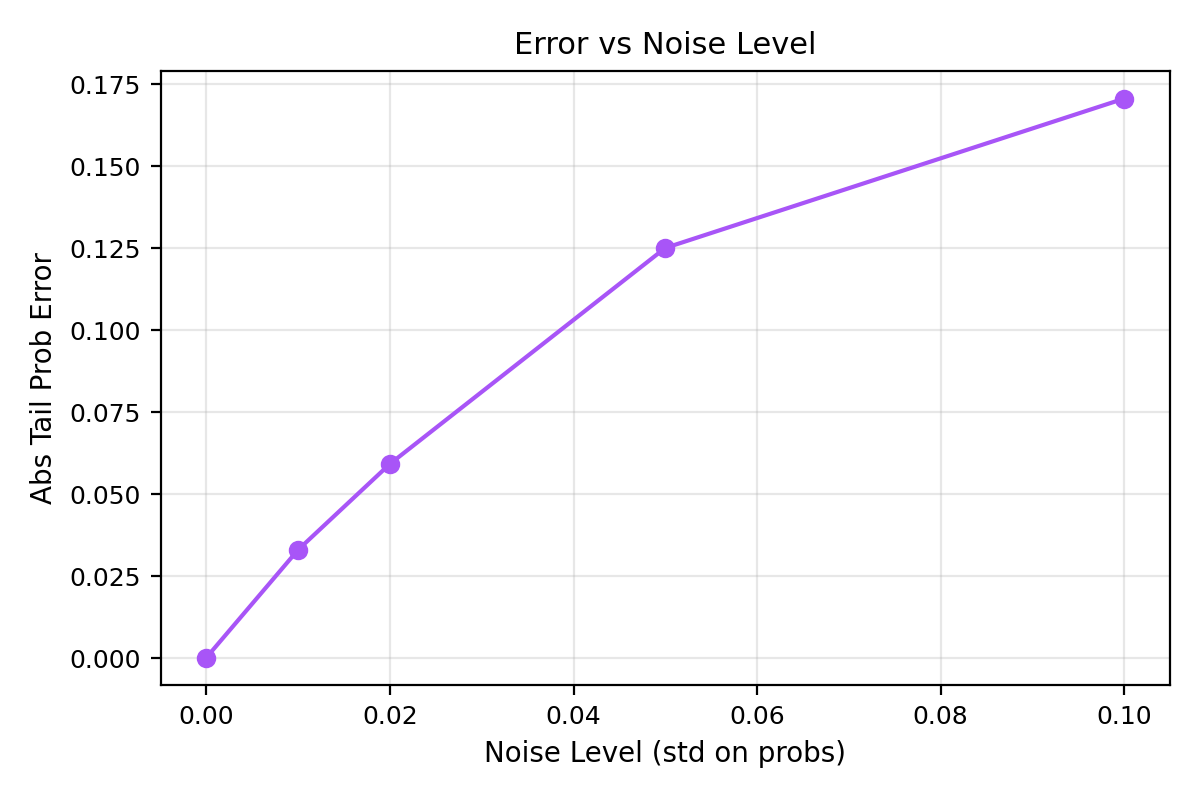
\includegraphics[width=\linewidth]{error_vs_noise_level.png}
    \\[-0.2em]
    {\scriptsize\colorbox{LogoPurple!15}{\strut Takeaway:} \emph{Noise ($\sigma\gtrsim0.05$) dominates error.}}
\end{minipage}
\end{center}
\end{block}

\end{column}

% Right column
\begin{column}{0.31\linewidth}

\begin{block}{Feasibility Boundary}
\begin{center}
    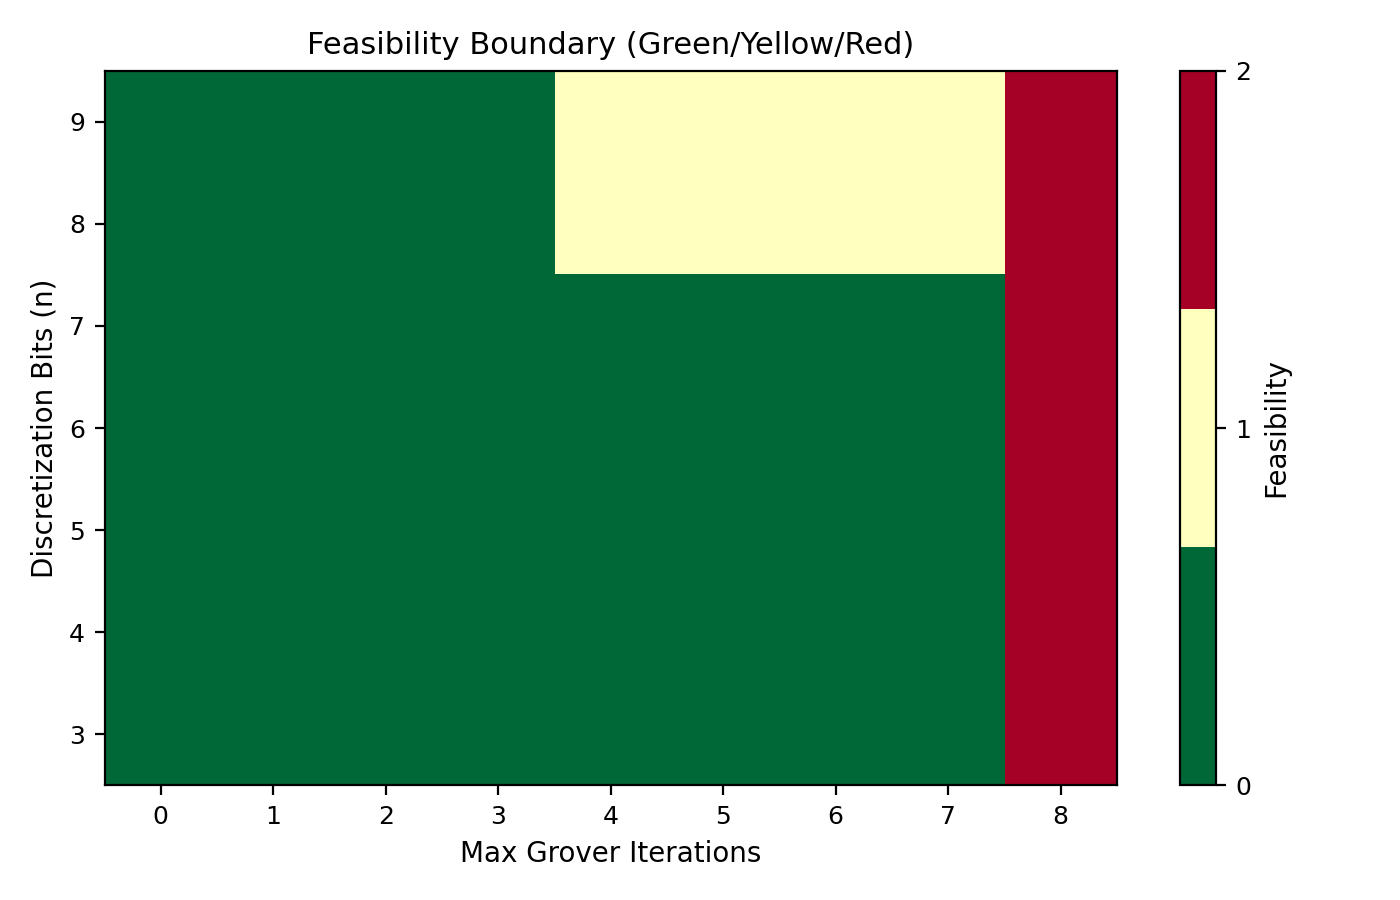
\includegraphics[width=0.85\linewidth]{feasibility_boundary.png}
\end{center}
In the \textcolor{ClassicGreen}{feasible region}, resource demands stay low enough for near-term devices, while the \textcolor{WarnYellow}{borderline region} signals settings that quickly become impractical. The \textcolor{WarnRed}{not-viable region} reflects NISQ-era limits where IQAE cost dominates the workflow. Bands use a composite resource score (qubits + depth + oracle calls).
\end{block}

\begin{block}{Dashboard Visuals}
Left panel collects portfolio inputs and stress settings; right panel reports VaR/CVaR, a tail-highlighted histogram, and a classical vs quantum comparison. IQAE reports the same tail probability with a confidence interval and absolute/relative error.
\begin{center}
\begin{minipage}[t]{0.49\linewidth}
    \centering
    \textbf{Classical Backend}\\[0.2em]
    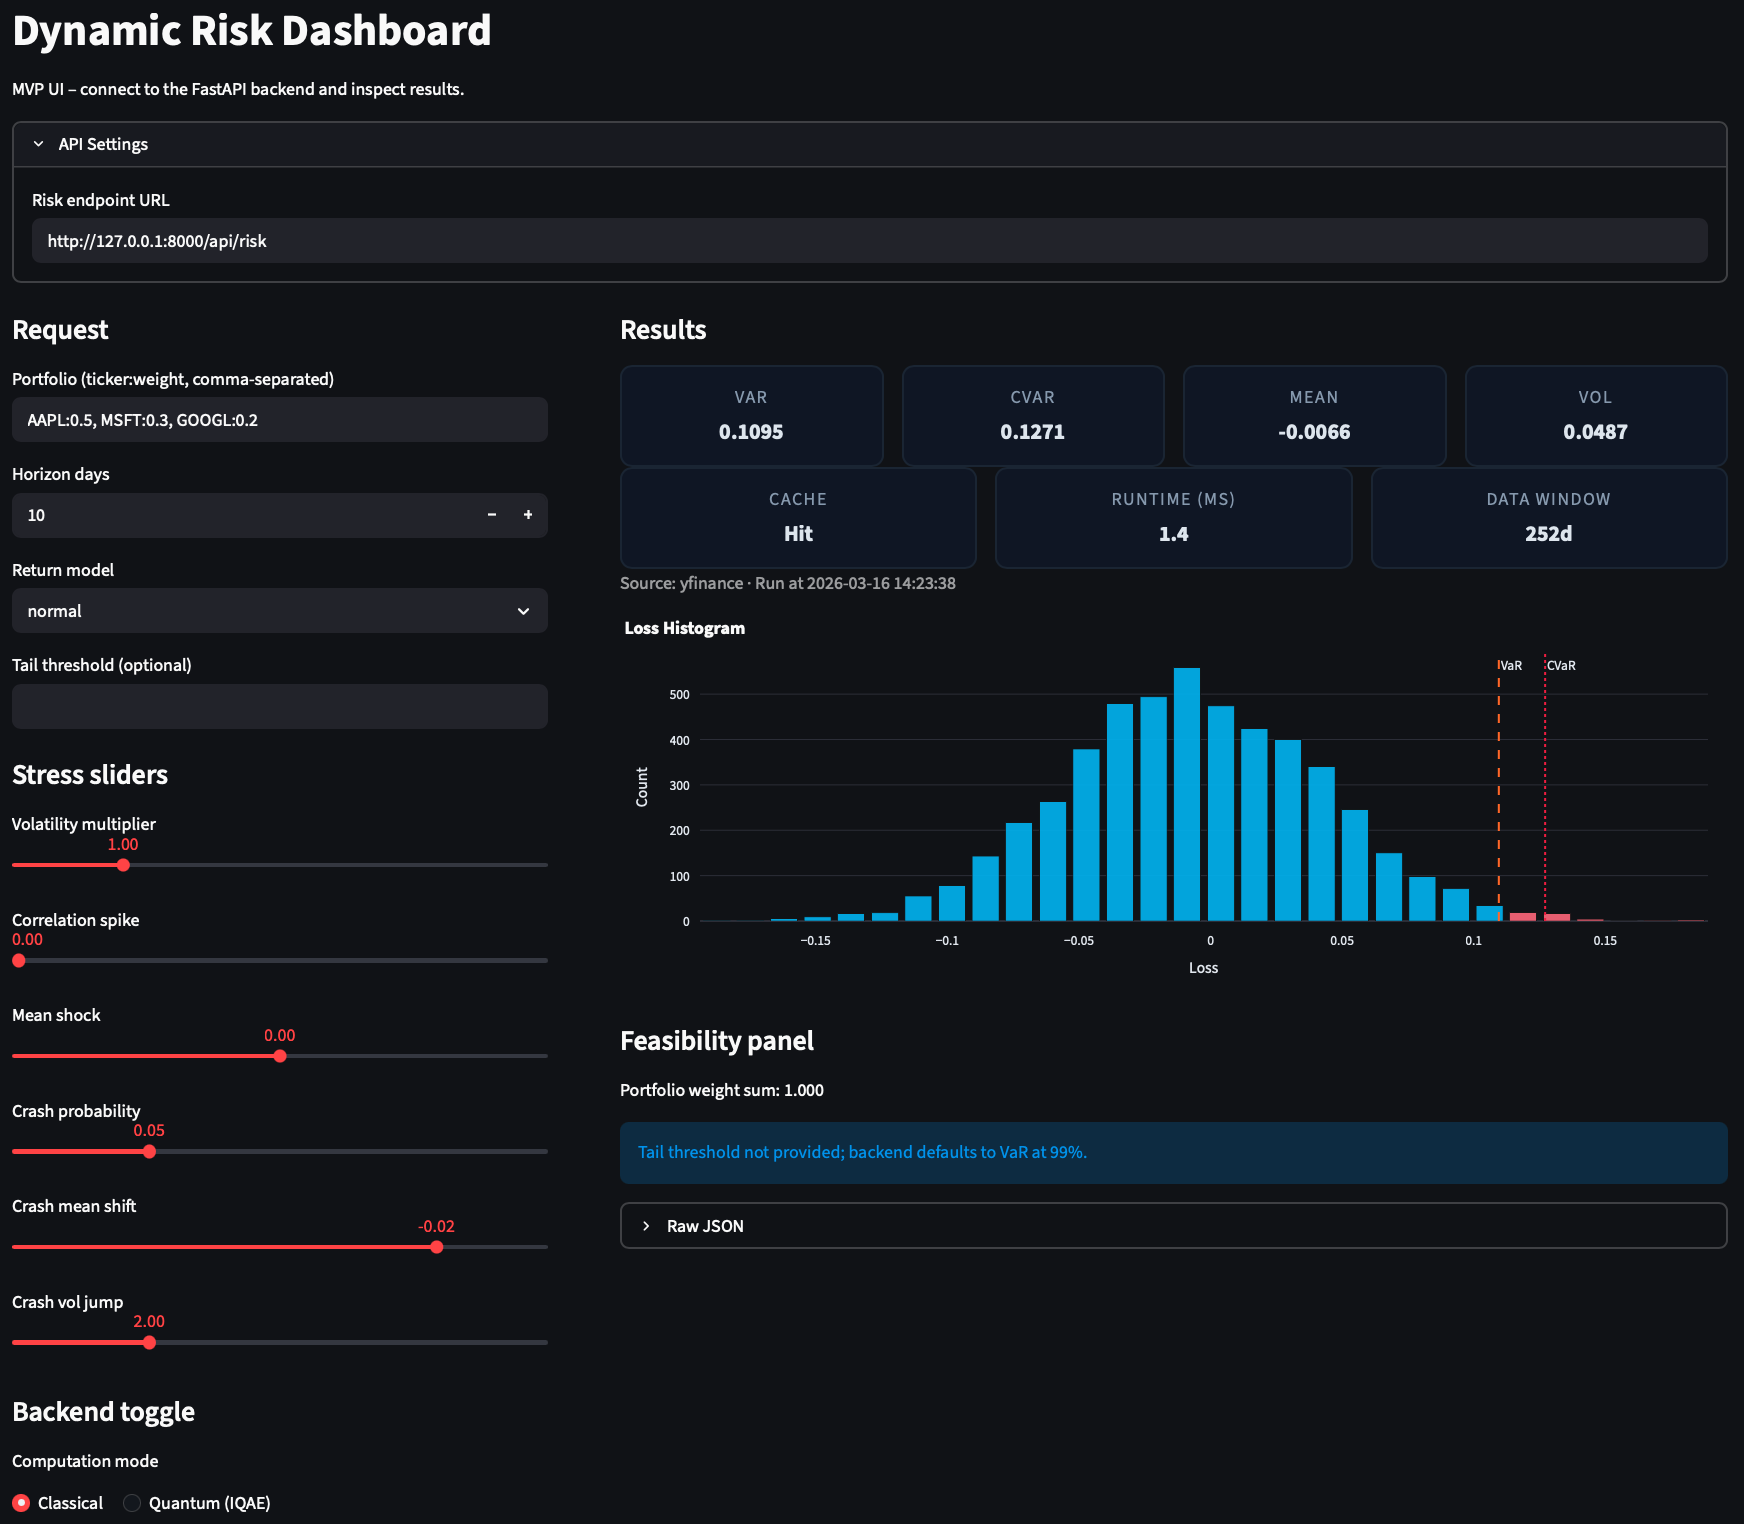
\includegraphics[width=\linewidth]{c_dash.png}
    \\[-0.2em]
    {\scriptsize\emph{Interpretability: tail-highlighted histogram with VaR/CVaR markers.}}
\end{minipage}\hfill
\begin{minipage}[t]{0.49\linewidth}
    \centering
    \textbf{Quantum (IQAE) Backend}\\[0.2em]
    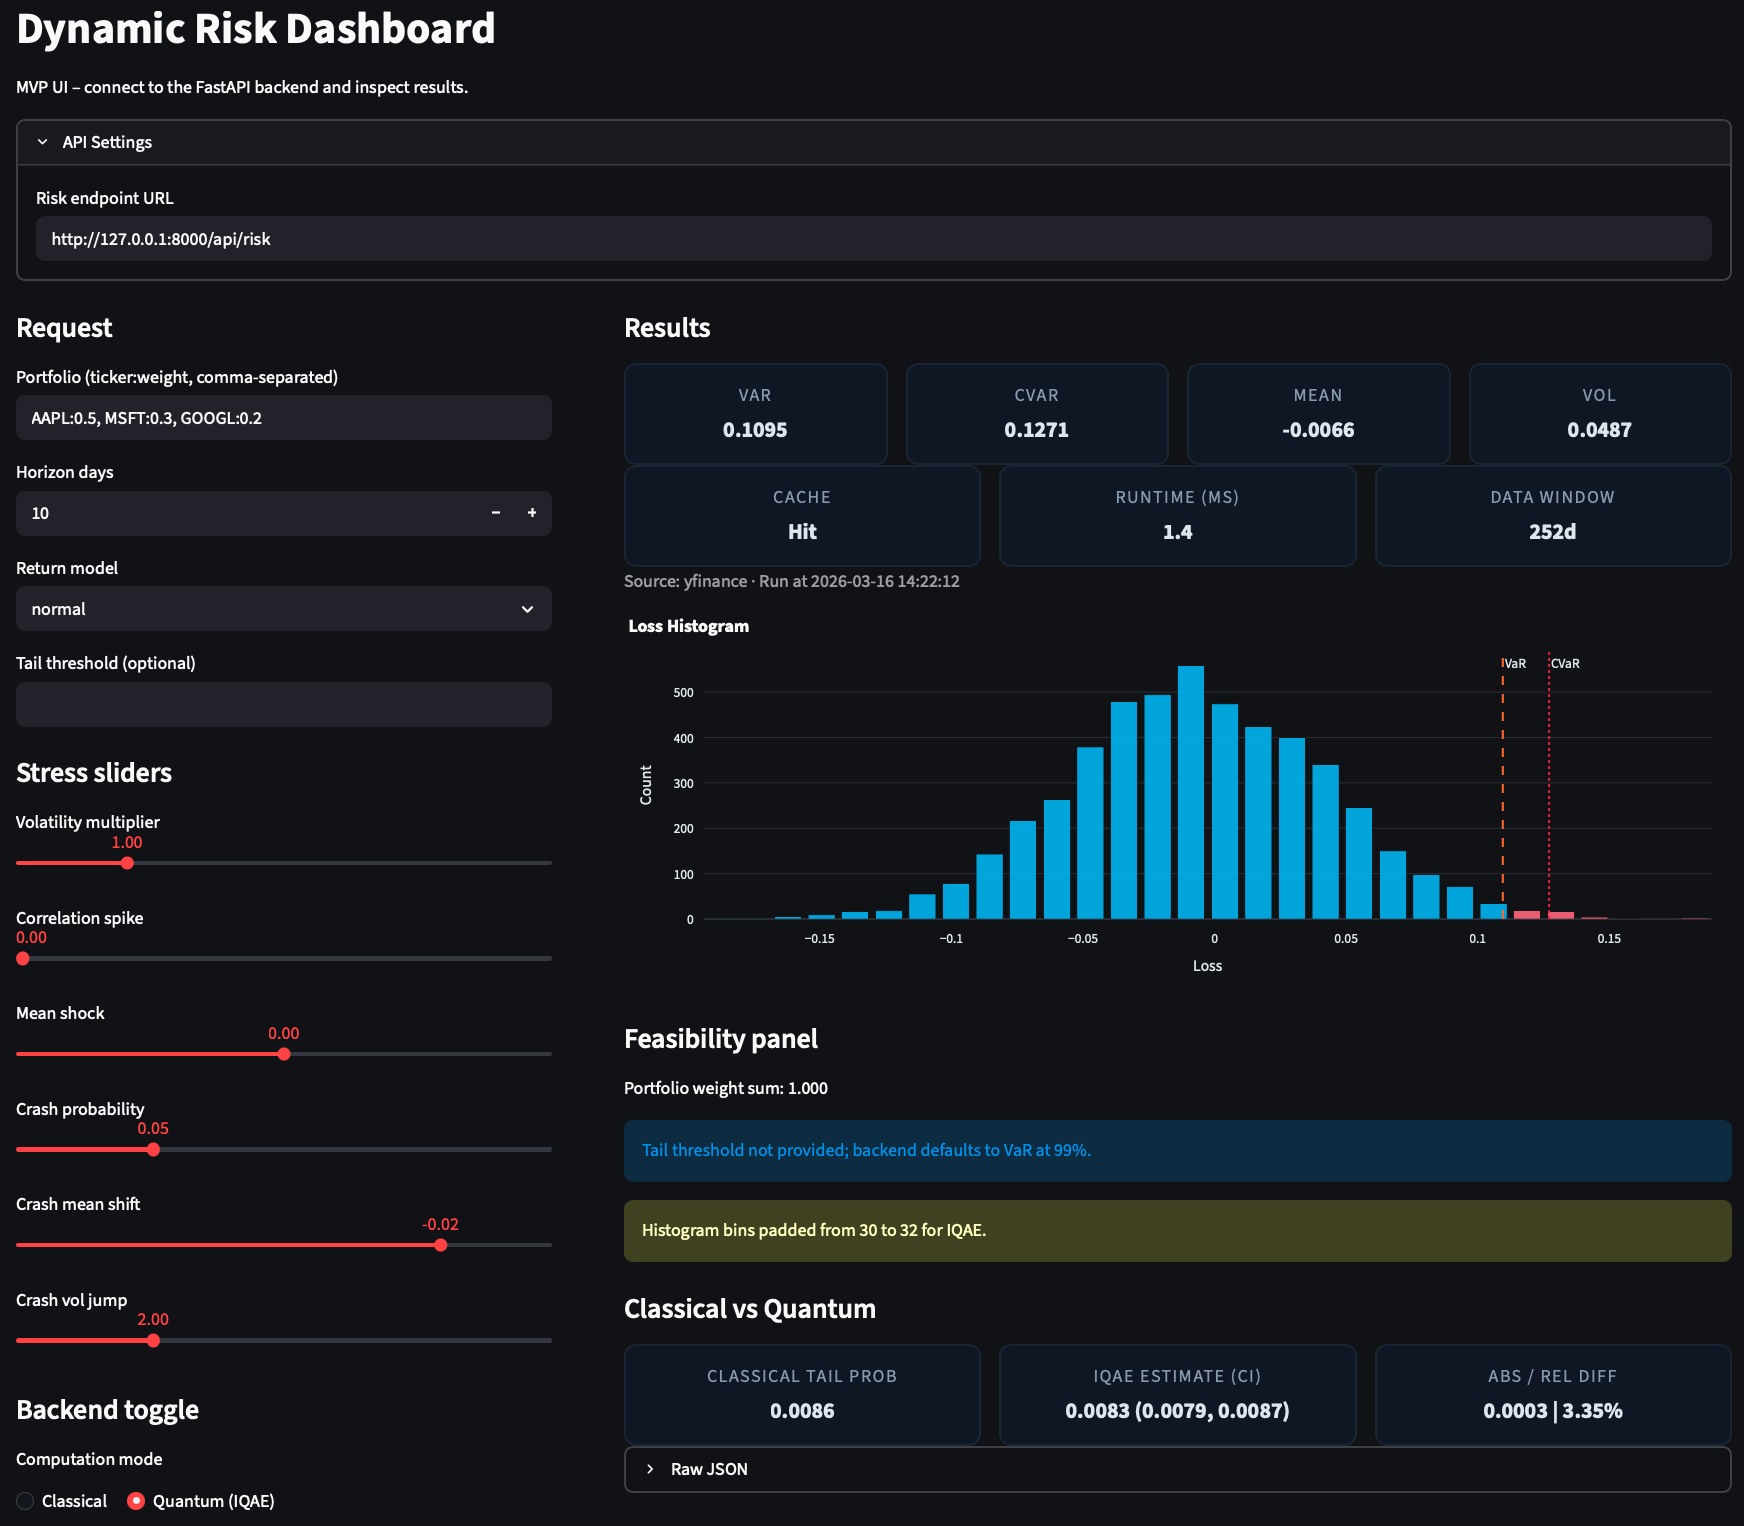
\includegraphics[width=\linewidth]{q_dash.png}
    \\[-0.2em]
    {\scriptsize\emph{Usability: IQAE CI + absolute/relative error vs classical.}}
\end{minipage}
\end{center}
\end{block}

\begin{block}{Discussion \& Implications}
\begin{itemize}
    \item Discretization provides a stable bridge to IQAE.
    \item Simulator estimates align with expected tail probabilities.
    \item Resource reports clarify near-term feasibility limits.
    \item Comparison uses the same threshold $\ell$, scenario, and histogram.
\end{itemize}
\end{block}

\begin{block}{Conclusion}
The MVP validates a classical-to-quantum risk pipeline with consistent inputs, interpretable outputs, and a clear audit trail from data to tail estimate.
\end{block}

\begin{block}{Acknowledgements \& Contact}
Western Quantum Club \quad Western University\\
\texttt{aorfali2@uwo.ca \quad eberling@uwo.ca}\\
\texttt{https://github.com/amirorfali/Dynamic-Risk-Dashboard}
\end{block}
\end{column}

\end{columns}
\end{frame}
\end{document}
